% ============
% Introduction
% ============
\section{Introduction} \label{introduction}

 Google Street View (GSV) has enabled millions of users to view street level imagery without having to visit locations in person. GSV has covered hundreds of cities in 20 countries over four continents by mounting camera systems on to vehicles that are able to capture panoramic images of an immediate surrounding \cite{Anguelov:2010}. These images provide a valuable source of geospatial data that can be difficult or expensive to obtain using aerial methods such as remote sensing, drones, or Light Detection and Ranging (LiDAR) \cite{Watts:2012}. Objects such as civilians, poles, and traffic signs viewed at the street level may be unidentifiable from an aerial view, but easily identified by users of GSV through visual inspection of street level imagery at particular locations. However, this task of manual inspection is time-consuming, tedious, and impractical for the massive quantities of imagery that are available. Computer vision techniques, namely object detection, can be used to automate the inspection of GSV image for the extraction of geo-located objects on a wide scale without requiring large amounts of manual labour.
 
 This paper detailed an experiment with a popular object detection method known as the Haar Cascade Classifier (HCC) on small subset of GSV images. The goal of the experiment was to extract the approximate location of stop signs in Toronto, Ontario for randomly selected GSV images. The experiment was done by first developing understanding of the HCC through a background review. A package was then developed to extract GSV images using an Application Programming Interface (API). A performance evaluation was done by manually labeling the small subset of extracted GSV images to observe the detection results. Finally, a discussion of challenges, proposed improvements, and future directions were provided to address the implications of the experiment.
 
 The proceeding sections are organized as follows:
 
\begin{itemize}
  \item Section \ref{background} details the HCC algorithm
  \item Section \ref{methods} details the methods used for extracting GSV images and performance evaluation
  \item Section \ref{results} presents the results of the performance evaluation
  \item Section \ref{discussion} discusses the experiment's challenges, proposed improvements, and future directions
  \item Section \ref{conclusion} provides concluding remarks and implications
\end{itemize}
 
% ==========
% Background
% ==========
\section{Background} \label{background}

This section provides background on the HCC algorithm. The HCC was based on the Viola and Jones algorithm, which provided an efficient object detection method for images using a machine learning approach \cite{Viola:2001}. The algorithm involves three main steps:

\begin{enumerate}
  \item \textbf{Feature creation}: abstraction of pixels into simple rectangular features
  \item \textbf{Learning classifiers}: learn function for feature selection based on lowest misclassification
  \item \textbf{Cascading classifiers}: negative sub-window rejection for efficient computation
\end{enumerate}

\subsection{Feature Creation} \label{feature-creation}

The feature creation process involves creating Haar-like features from pixels in an image. Haar-like features are simple rectangular features computed from individual image pixels. Integral images are used to efficiently create Haar-like features from images by computing rectangular sums in constant time. This section provides details on Haar-like features and integral images for object detection in images.

\subsubsection{Haar-like Features} \label{haar-like-features}

Haar-like features form abstract representations of individual pixels from a grayscale image. For example, a rectangular region of an image can contain an abstract representation such as a line or an edge, which is defined by the gradient changes between light and dark pixels. The dimensions of each rectangular region are defined by the user, where 24 by 24 regions are suggested as optimal through empirical observation \cite{Viola:2001}. In addition to the rectangular regions, Haar-like features consist of additional rectangular sub-regions with aggregated pixel values to capture a simplified structure. Each sub-region containing individual pixels can be either white or black, where the sum of the white regions subtracted from the sum of the black regions produce a single value to be used for object detection. A sliding window, representing a rectangular region, is used to capture these sub-regions throughout the image to compute single values representing features for each image.

\begin{figure}[htb]
  \begin{subfigure}[t]{2in}
    \centering
    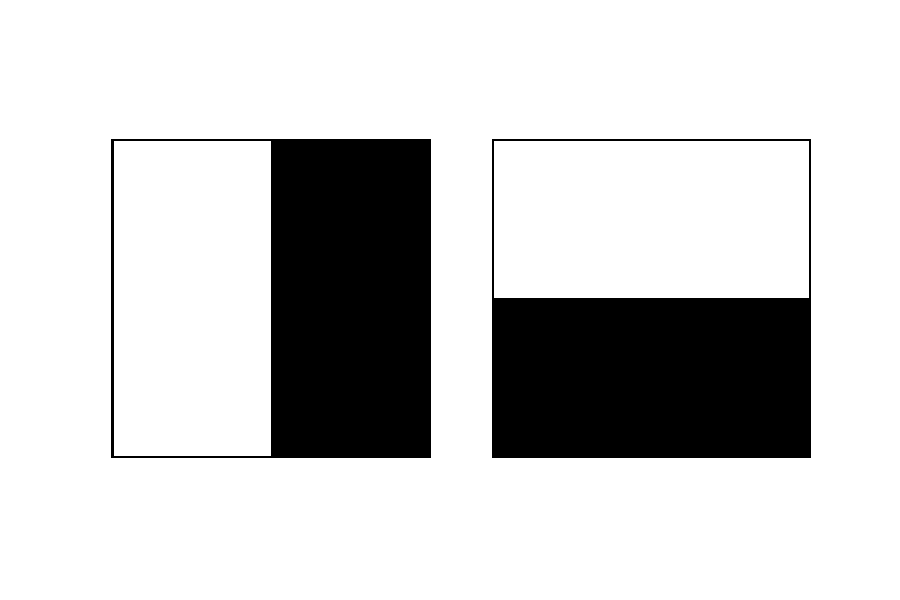
\includegraphics[height=1.5in]{haars_papageogiou}
    \caption{Two Rectangle}
  \end{subfigure}
  \hfill
  \begin{subfigure}[t]{2in}
    \centering
    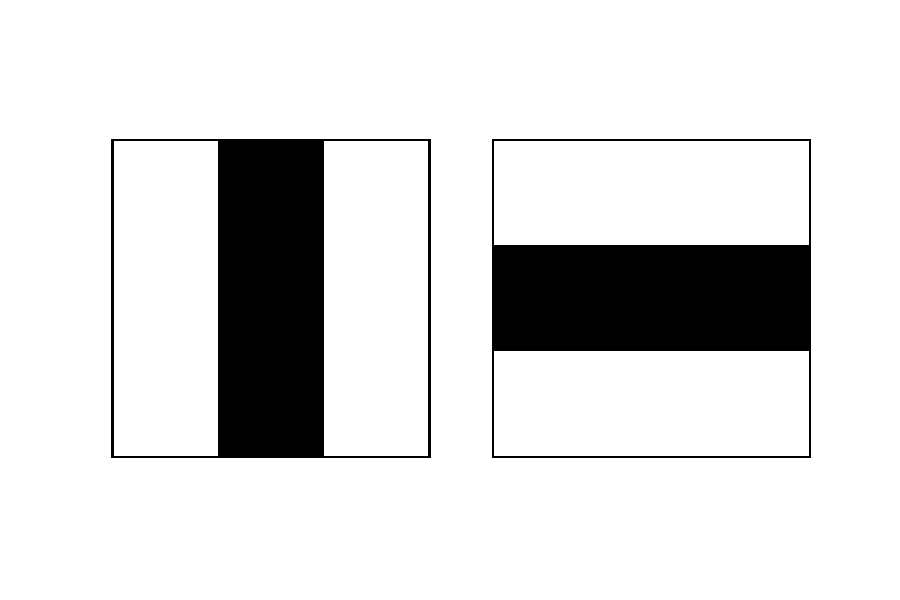
\includegraphics[height=1.5in]{haars_violajones}
    \caption{Three Rectangle}
  \end{subfigure}
  \hfill
  \begin{subfigure}[t]{2in}
    \centering
    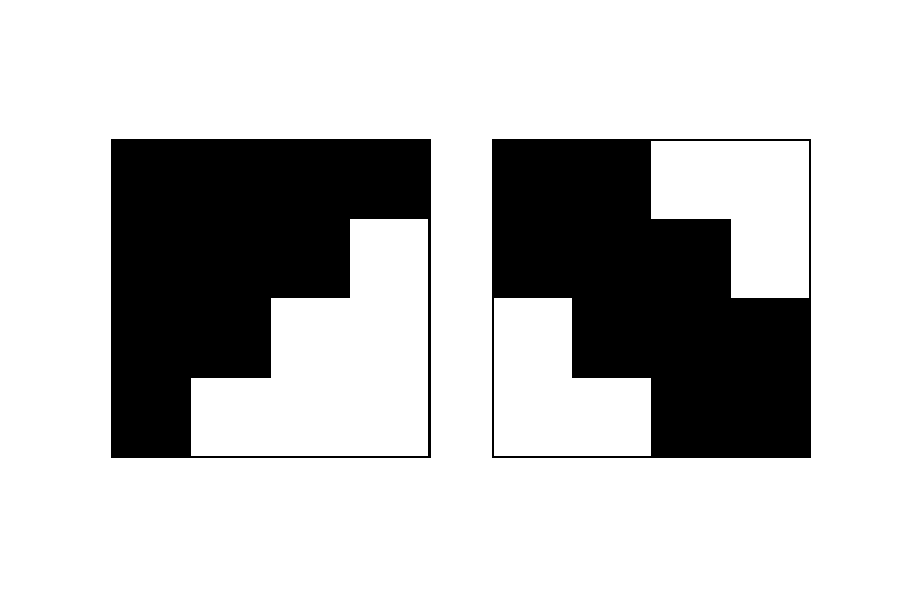
\includegraphics[height=1.5in]{haars_lienmaydt1}
    \caption{Rotated}
  \end{subfigure}
  \hfill
  \begin{subfigure}[t]{2in}
    \centering
    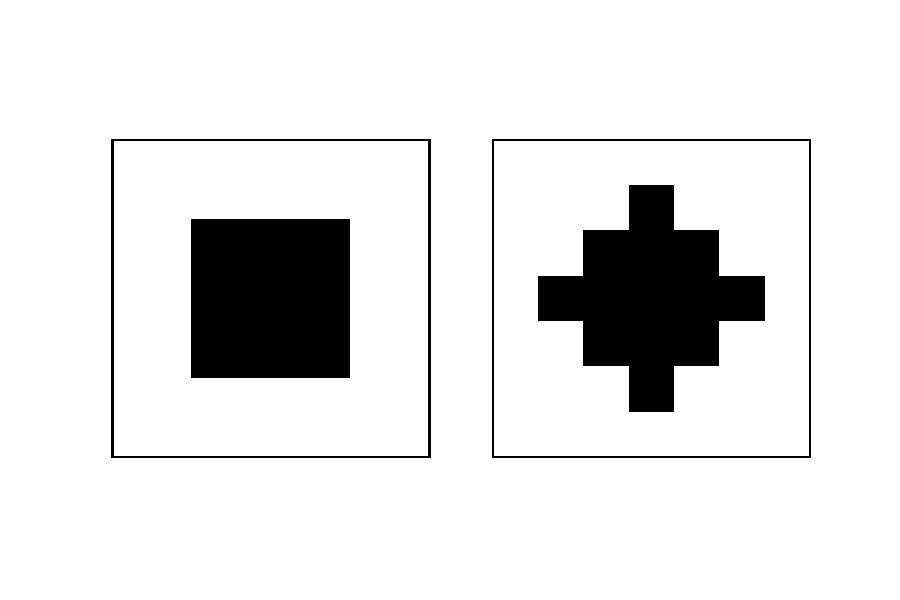
\includegraphics[height=1.5in]{haars_lienmaydt2}
    \caption{Center-surround}
  \end{subfigure}
  \caption{Haar-like features}
  \label{fig:haars}
\end{figure}

Several haar-like features have been proposed to be effective for object detecton. Simple two-rectangle features \cite{Papageorgiou:1998}, three rectangle features in \cite{Viola:2001}, rotated features, and center-surround features \cite{Lienhart:2002} are seen in Figure \ref{fig:haars}. These features can be used to abstract details in images to represent identifying features of objects such as noses, where a three-rectangle feature can be used to measure the grayscale contrast of the lighter region on a nose, and darker regions to both sides of a nose.

\subsubsection{Integral Images} \label{haar-like-features}

Integral images (also known as summed area tables) are pre-computed to efficiently calculate sums in rectangular regions of an image \cite{Crow:1984}. An integral image is created by inclusively summing each pixel in the original image by the pixels that are to the left and above as seen in Equation \ref{eq:integral-image}.

\begin{equation} \label{eq:integral-image}
  ii(x, y) = \sum_{x_i \leq x, y_i \leq y}{i(x_i, y_i)}
\end{equation}

where $ii(x,y)$ is the integral image at row $x$ and column $y$, and $i(x_i, y_i)$ is the original image pixels that are to the left and above $ii(x,y)$. The sum of rectangular regions can be then be efficiently calculated using the pixel values of the pre-computed integral image.

A rectangular region is defined by a pair of top-left and bottom-right corner coordinates seen in Equation \ref{eq:rectangle}:

\begin{equation} \label{eq:rectangle}
(x_1, y_1), (x_2, y_2)
\end{equation}

where $(x_1, y_1)$ are the top-left coordinates of the rectangular region, and 
$(x_2, y_2)$ are the bottom-right coordinates of the rectangular region.

Four integral image pixel values relative to the top-left and bottom-right coordinates of the rectangular region are defined by Equations \ref{eq:A} to \ref{eq:D}:

\begin{equation} \label{eq:A}
A = ii(x_1 - 1, y_1 - 1)
    \begin{cases}
        0: \text{if} & x_1 - 1 \not\in \left\{ x_{min} \dots x_{max} \right\} \\
        0: \text{if} & y_1 - 1 \not\in \left\{ y_{min} \dots y_{max} \right\} \\
    \end{cases}
\end{equation}

\begin{equation} \label{eq:B}
B = ii(x_2, y_1 - 1)
    \begin{cases}
        0: \text{if} & x_2 \not\in \left\{ x_{min} \dots x_{max} \right\} \\
        0: \text{if} & y_1 - 1 \not\in \left\{ y_{min} \dots y_{max} \right\} \\
    \end{cases}
\end{equation}

\begin{equation} \label{eq:C}
C = ii(x_1 - 1, y_2)
    \begin{cases}
        0: \text{if} & x_1 - 1 \not\in \left\{ x_{min} \dots x_{max} \right\} \\
        0: \text{if} & y_2 \not\in \left\{ y_{min} \dots y_{max} \right\} \\
    \end{cases}
\end{equation}

\begin{equation} \label{eq:D}
D = ii(x_2, y_2)
    \begin{cases}
        0: \text{if} & x_2 \not\in \left\{ x_{min} \dots x_{max} \right\} \\
        0: \text{if} & y_2 \not\in \left\{ y_{min} \dots y_{max} \right\} \\
    \end{cases}
\end{equation}

where if the coordinates $x_1, y_1, x_2, y_2$ are outside the $x_{min}, y_{min}, x_{max}, y_{max}$ dimensions of the integral image $ii$, then the value will be 0, otherwise the respective pixel values from $ii$ of $A, B, C, D$ are assigned.

The sum of the pixel values inside the original image is given by Equation \ref{eq:integral-sum}:

\begin{equation} \label{eq:integral-sum}
S_i(x_1, y_1, x_2, y_2) = D - B - C + A
\end{equation}

where $S_i(x_1, y_1, x_2, y_2)$ is the sum of all pixel values of the original image $i$ inside the rectangular region, which is defined by the top-left coordinates $x_1, y_1$ and bottom-right coordinates $x_2, y_2$.

The brute force method for the sum of all pixels inside the rectangular region requires the access of $n$ pixels inside the rectangular region ($O(n)$), while the integral image enables the sum to be computed by at most 4 pixel accesses in the integral image at constant time ($O(1)$). The integral images can be used to process Haar-like features efficiently as two-rectangle features require at most 8 pixel accesses, and three-rectangle features require at most 12 accesses for features of any dimension. A detailed example of calculating integral images is provided in Appendix \ref{integral-image-example}.

\subsection{Learning Classifiers} \label{learning classifiers}

A machine learning algorithm known as Adaboost was used to learn classifiers for feature selection. Machine learning algorithms seek to optimize performance measures by learning from examples, known as training data, to generalize on new examples not seen in the learning process \cite{Domingos:2012}. Classifiers are models generated by machine learning algorithms to determine whether the input data belongs to one or more known categories (classes) \cite{Kotsiantis:2006}. Adaboost combines several weak classifiers, using a process called boosting, to create a strong classifier \cite{Freund:1997, Schapire:1999}. Weak classifiers are algorithms that perform slightly better than random guessing (for example, classifying a data sample correctly more than 50\% of the time). These weak classifiers are combined to produce a strong classifier, which performs better than the individual weak classifiers, using a process called \textit{boosting}. Boosting refers to iteritively learning weak classifiers using a vector of weights, where the weights are re-calculated based on performances of previous weak classifiers.

A set of example images, their feature values, and their label (positive or negative) are given by Equation \ref{eq:adaboost-input}: 

\begin{equation} \label{eq:adaboost-input}
(x_i, f_{i, j}, y_i) \ \text{for} \ i \dots n_i \ \text{and} \ j \dots n_j \text{, such that} \ y_i \in \left\{0, 1 \right\}
\end{equation}


where $x_i$ is example image $i$, $f_{i, j}$ is feature $j$ for image $i$, $y_i$ are the labels for example image $i$ (0 being negative and 1 being positive), $n_i$ is the number of example images, and $n_j$ is the number of features for $xi$.

A set of weights are initialized for each of the example images seen in Equation \ref{eq:weights}:

\begin{equation} \label{eq:weights}
w_{1,i} = 
    \begin{cases}
        \frac{1}{2m}: \text{if} \ y_i = 0 \\
        \frac{1}{2l}: \text{if} \ y_i = 1\\
    \end{cases}
\end{equation}

where $m$ is the number of negative example images, and $l$ is the number of positive images.

The HCC is based on a modified version of Adaboost, in which the following equations are applied for $t$ number of iterations until a specified criteria is met (such as reaching the desired classification accuracy or optimizing the misclassification error).

Create a probability distribution of normalized weights $w_{t,i}$, for each $t$, such that $w_{t,i}$ is in the range of 0 to 1 and sums to 1 as seen in Equation \ref{eq:normalize}:

\begin{equation} \label{eq:normalize}
w_{t,i} = \frac{w_{t,i}}{\sum_{k=1}^{n_i}{w_{t,k}}}
\end{equation}
    
where $n_i$ is the number of example images, and $\sum_{k=1}^{n_i}{w_{t,k}}$ is the sum of the weights for all images.

Train a weak classifier $h_j(x)$ for each feature $j$ using example images $xi$ and their labels $yi$. Viola and Jones uses a decision stump as the weak classifier defined in Equation \ref{eq:weak-classifier}:

\begin{equation} \label{eq:weak-classifier}
h(x, f, p, \theta) = 
\begin{cases}
  1: \text{if} \ p \ f(x) \lt p \theta \\
  0: \text{otherwise} \\
\end{cases}
\end{equation}

where $h(x)$ is the weak classifier for a feature given example image $x$ defined by a sub-window (such as a 24 by 24 rectangular sub-region), $p$ is the parity representing the direction of the inequality sign (positive or negative), $f(x)$ is the single value for the rectangular feature of $x$, and $\theta$ is a threshold. The threshold $\theta$ is learned by training a decision stump to first order the feature values $f$ from lowest to highest for each image $x$, followed by selecting the feature value that optimizes $h$ for the lowest error measure defined by Equation \ref{eq:error}:

\begin{equation} \label{eq:error}
e = \min(S^+ + (T^- - S^-), S^- + (T^+ - S^+))
\end{equation}

where $S^+$ is the sum of positive weights below the current feature value $f$, $S^-$ is the sum of negative weights below the current feature value $f$, $T^+$ is the total sum of all positive example weights, and $T^-$ is the total sum of all negative example weights. This error can be interpreted as a measure of the minimum error of labeling examples below a feature value and above a feature value given the weights \cite{Viola:2004}. The feature value with the minimum error $e$ is then selected as the threshold $\theta{_j}$.

Choose the classifier $h_j$ with the lowest error $\epsilon_j$ defined by Equation \ref{eq:error2}:
    
\begin{equation} \label{eq:error2}
\epsilon_j = \sum_i^n{w_i \left\lvert h_j(x_i, f_j, p, \theta_j) - y_i \right\rvert}
\end{equation}

where $h_j(x_i, f_j, p, \theta_j)$ is the predicted label (0 negative or 1 for positive), and $y_i$ is the true label. 

The classifier with the lowest error $h_t$ minimizes $\epsilon_j$ by optimizing $\theta_j$ and $p$ shown in Equation  \ref{eq:minimize}:

\begin{equation} \label{eq:minimize}
\min_{\theta_j \ \in \ \mathbb{R}, \ p \ \in \ \left\{ +1,-1 \right\}}\epsilon_j(x_i, f_j, p, \theta_j)
\end{equation}

The weights are updated after selecting the classifier $h_j$ using the Equation \ref{eq:update}:
    
\begin{equation} \label{eq:update}
w_{t+1,i} = w_{t,i} \beta_t^{1-e_j}
\end{equation}
    
where $\beta_t$ is $\frac{\epsilon_t}{1-\epsilon_t}$.

After $t$ iterations, a final strong classifier $C(x)$ can then be formed using Equation \ref{eq:strong-classifier}:

\begin{equation} \label{eq:strong-classifier}
C(x) = 
\begin{cases}
    1: \text{if} \ \sum_{t=1}^T{\alpha_t h_t(x) \geq \frac{1}{2} \sum_{t=1}^T{\alpha_t}} \\
    0: \text{otherwise} \\
\end{cases}
\end{equation}

where $\alpha_t = \log \frac{1}{B_t}$, and $h_t$ are the weak classifiers learned from $t$ iterations. This strong classifier is the combination of the weak classifiers such that the predictions are the weighted majority votes.

\subsection{Cascading Classifiers} \label{cascading-classifiers}

A cascade of classifiers was used in the Viola and Jones algorithm to reduce the number of rectangular regions (sub-windows) that need further processing, and to improve the detection rate \cite{Viola:2004}. A cascade of classifiers is constructed using the Adaboost algorithm. A cascade consists of several stages that increase the detection rate and false positive rate with a higher number of stages. In order for a rectangular region to be further processed, it has to pass each stage of the cascade. If the rectangular region is classified as negative at any stage, it is rejected immediately and further processing is stopped. Each stage of a cascade classifier uses the previous stage's examples that were successfully passed as positive, which makes subsequent stages inherit increasingly difficult examples that form classifiers with with rules that are more strict. The number of stages depend on the desired detection or false positive rate set manually by the user.

The detection rate of a cascade $D$ is given by Equation \ref{eq:detection}:

\begin{equation} \label{eq:detection}
D = \prod_{t=1}^K d_i
\end{equation}

where $K$ is the number of classifiers and $d_i$ is the detection rate of classifier $i$ on examples that are accepted by it. 

The false positive rate of a cascade $F$ is given by Equation \ref{eq:false-positive}:

\begin{equation} \label{eq:false-positive}
F = \prod_{t=1}^K f_i
\end{equation}

where $K$ is the number of classifiers and $f_i$ is the false positive rate of classifier $i$ on examples that are accepted by it. 

% =======
% Methods
% =======
\section{Methods} \label{methods}

This section describes the procedures taken to perform the experiment of a stop sign detection HCC for GSV images. A set of positive and negative images were required to evaluate a Haar Cascade Classifier for stop signs. Positive images are example images that contain the object to be detected, and negative images are example images that do not contain the object to be detected. The positive and negative images were extracted by locating stop signs from OpenStreetMap, and querying Google Street View using those locations \cite{Haklay:2008}. The data was then manually inspected to be labelled as positive or negative, and was used for performance evaluation. The procedure involved four major steps:

\begin{enumerate}
  \item \textbf{Locating stop signs}: extraction of stop sign locations using OpenStreetMap
  \item \textbf{Extracting Google Street View Images}: extraction of GSV images using stop sign locations
  \item \textbf{Stop Sign Detection Model}: utilize a pre-trained HCC model for performance evaluation of the GSV images
  \item \textbf{Performance Evaluation}: evaluate correct detections and false positives using the GSV images
\end{enumerate}

\subsection{Locating Stop Signs} \label{locating-stop-signs}

\begin{figure}[H]
\begin{framed}
\begin{verbatim}
[out:json];
node[highway=stop]
  (43.458297,-79.639219,43.8554579,-79.002481);
out;
\end{verbatim}
\end{framed}
\caption{Overpass API query for stop sign locations}
\label{fig:query}
\end{figure}

The location of stop signs were extracted using the Overpass API through a Uniform Resource Location (URL) link with a data query string \cite{OpenStreetMap:2017, Lee:1994}. The Overpass API provided OpenStreetMap data by enabling users to send requests made of queries to filter desired data subsets. Details on the Overpass API URL structure is available in Appendix \ref{overpass-api-url-structure}. 

The stop sign locations were limited to Toronto, Ontario, by specifying a bounding box defined by 43.458297 and -79.639219 (latitude and longitude of the bottom left corner), and 43.8554579 and -79.002481 (latitude and longitude of the top right corner). Stop signs were tagged as \textit{highway=stop} on OpenStreetMap, and locations were known as \textit{nodes}. The Overpass API query is shown in Figure \ref{fig:query}, which was used to produce the final URL to extract the stop sign locations \cite{OpenStreetMap:2017}. For the purpose of this experiment, 99 locations were randomly selected to be used as a small subset of data.

\subsection{Extracting Google Street View Images} \label{extracting-google-street-view-images}

\begin{figure}[H]
\begin{framed}
\begin{verbatim}
size=640x640
location="location_of_stop_sign1..n"
fov=120
key="developer_key"
\end{verbatim}
\end{framed}
\caption{Google Street View API base query}
\label{fig:gsvquery}
\end{figure}

GSV images were collected using the stop sign locations in Section \ref{locating-stop-signs}. A Python package named \textit{google\_streetview} was developed to create data query strings for the GSV API and automatically download GSV image requests \cite{Wen:2017}. The available GSV API parameters to be set by the user are shown in Table \ref{table:gsvapi}. Figure \ref{fig:gsvquery} shows the parameters used to extract each GSV image using the stop sign locations. Each location parameter was replaced by a location from the randomly selected stop sign locations. Details on the GSV API URL structure is available in Appendix \ref{google-street-view-url-structure}.

\begin{table}
\begin{center}
\begin{tabular}{ | p{5cm} | p{5cm} |}
\hline
\textbf{Parameter} & \textbf{Description} \\ 
\hline
location or pano & coordinates (latitude, longitude) or address \\ 
\hline
key & the google developer key \\ 
\hline
heading &  compass rotation of camera from 0 to 360 degrees (the default directs it to face the location)\\ 
\hline
fov & horizontal field of view from 0 to 120 (default is 90) \\
\hline
pitch & vertical angle of camera from -90 to 90 with 0 being in the middle (the default is 0) \\
\hline
size & image size up to 640 by 640\\
\hline
\end{tabular}
\caption{Google Street View Paramters}
\label{table:gsvapi}
\end{center}
\end{table}

\subsection{Stop Sign Detection Model} \label{stop-sign-detection-model}

\begin{figure}[H]
  \begin{subfigure}[t]{1.5in}
    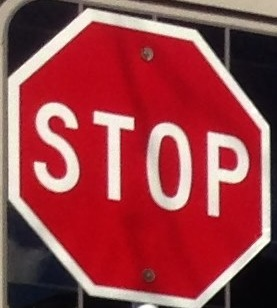
\includegraphics[height=1.5in]{train_positive_01}
  \end{subfigure}
  \hfill
  \begin{subfigure}[t]{1.5in}
    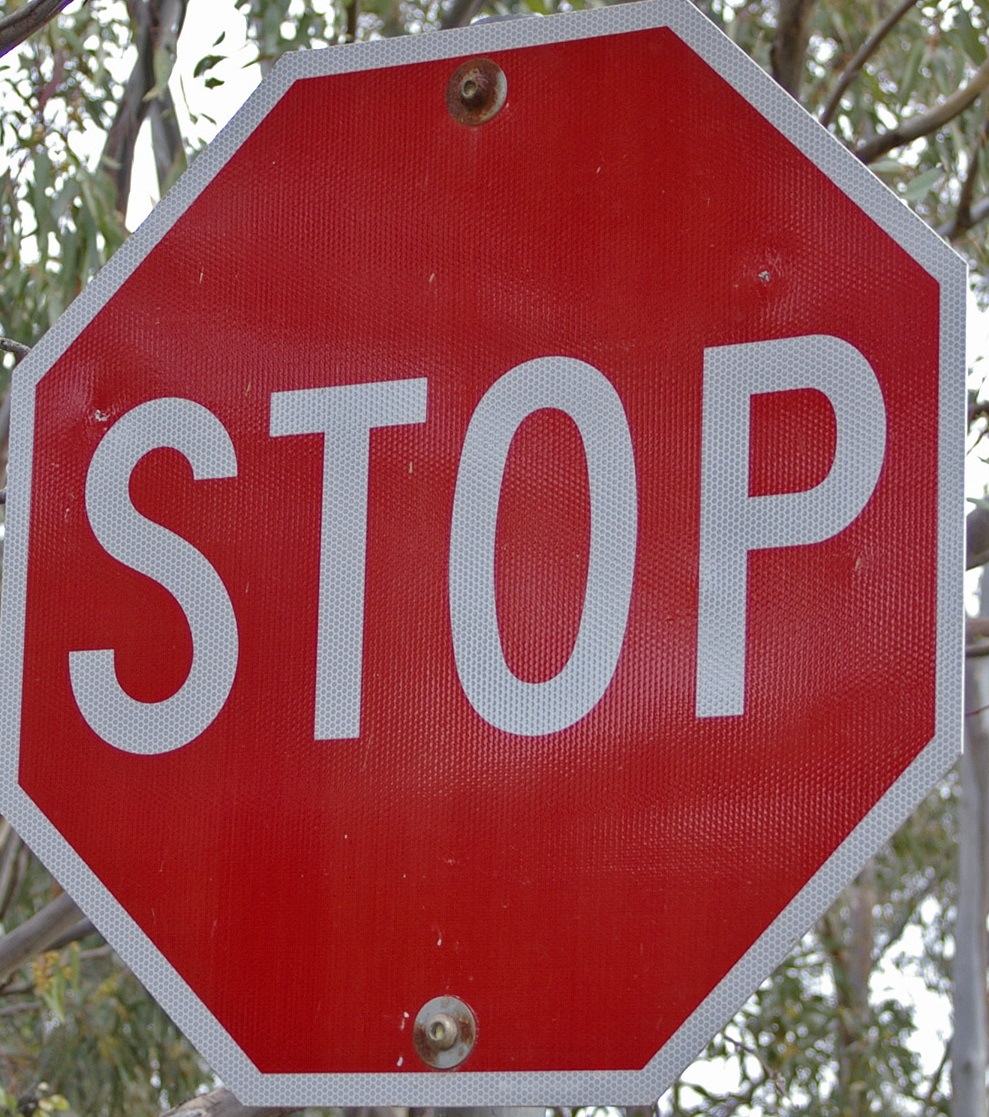
\includegraphics[height=1.5in]{train_positive_08}
  \end{subfigure}
  \hfill
  \begin{subfigure}[t]{1.5in}
    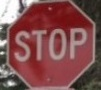
\includegraphics[height=1.5in]{train_positive_28}
  \end{subfigure}
  \par\bigskip
  \begin{subfigure}[t]{1.5in}
    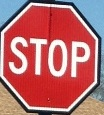
\includegraphics[height=1.5in]{train_positive_38}
  \end{subfigure}
  \hfill
  \begin{subfigure}[t]{1.5in}
    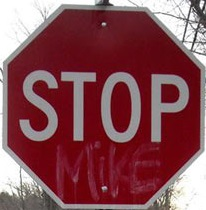
\includegraphics[height=1.5in]{train_positive_71}
  \end{subfigure}
  \hfill
  \begin{subfigure}[t]{1.5in}
    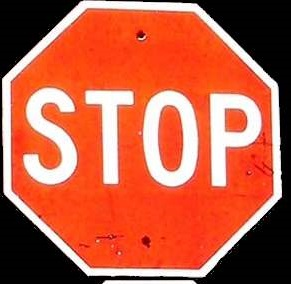
\includegraphics[height=1.5in]{train_positive_80}
  \end{subfigure}
  \caption{Example of positive training images}
  \label{fig:train-positive}
\end{figure}

\begin{figure}[H]
  \begin{subfigure}[t]{1.5in}
    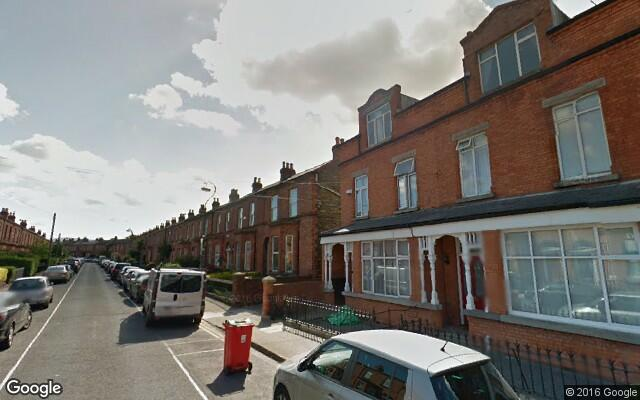
\includegraphics[height=1in]{train_negative_01}
  \end{subfigure}
  \hfill
  \begin{subfigure}[t]{1.5in}
    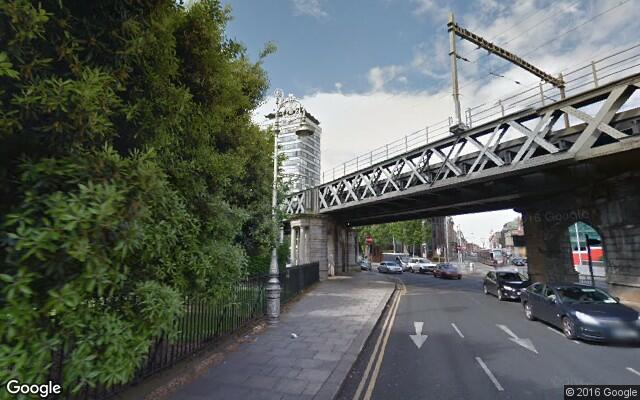
\includegraphics[height=1in]{train_negative_02}
  \end{subfigure}
  \hfill
  \begin{subfigure}[t]{1.5in}
    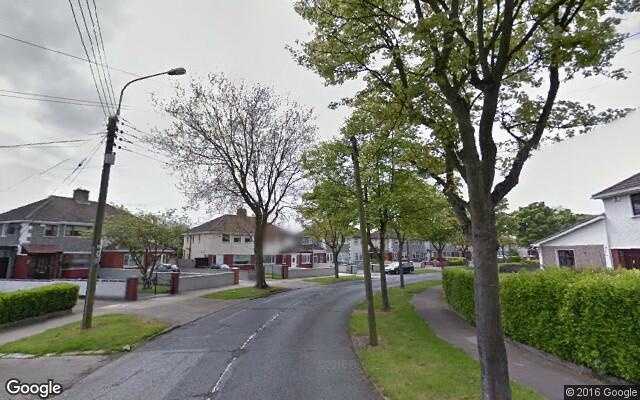
\includegraphics[height=1in]{train_negative_03}
  \end{subfigure}
  \par\smallskip
  \begin{subfigure}[t]{1.5in}
    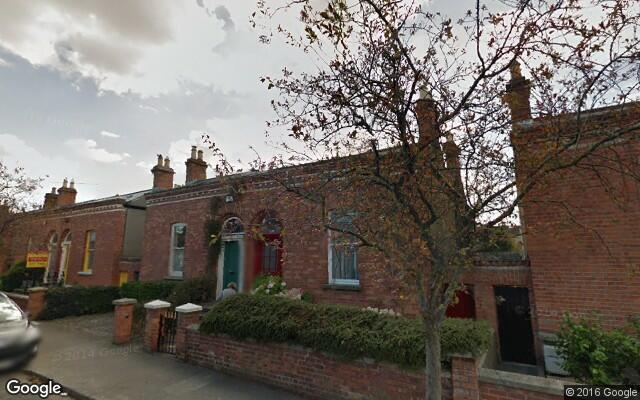
\includegraphics[height=1in]{train_negative_13}
  \end{subfigure}
  \hfill
  \begin{subfigure}[t]{1.5in}
    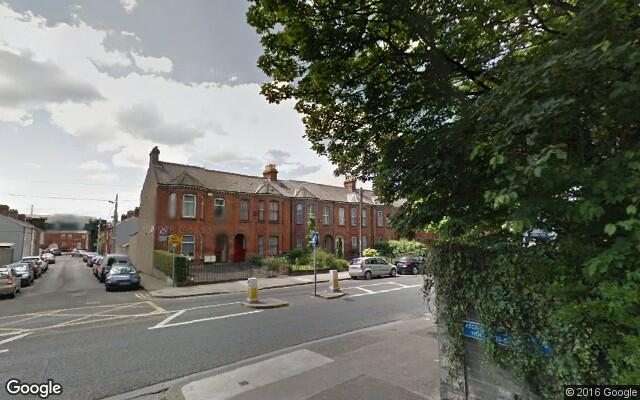
\includegraphics[height=1in]{train_negative_14}
  \end{subfigure}
  \hfill
  \begin{subfigure}[t]{1.5in}
    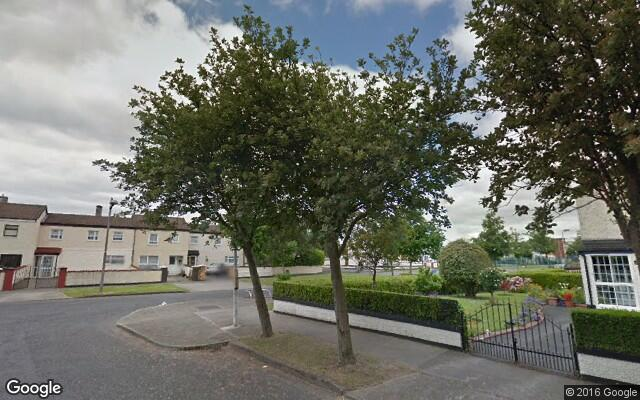
\includegraphics[height=1in]{train_negative_15}
  \end{subfigure}
  \caption{Example of negative training images}
  \label{fig:train-negative}
\end{figure}

A HCC model was trained on 82 images of stop signs, and 1115 images of surrounding street backgrounds\footnote{The HCC file and training images were made available thanks to user \textit{markgaynor} on Github under the MIT license}. The 82 images of stop signs are known as the positive training data, and the 1115 images of surrounding street backgrounds were known as the negative training data. Additional samples were also created from the training data by iteritively applying distortions to account for stop signs that were viewed from different angles. Figure \ref{fig:train-positive} shows the positive training images, and Figure \ref{fig:train-negative} shows the negative training images.

\subsection{Performance Evaluation} \label{performance-evaluation}

The 99 GSV images extracted from the GSV API (described in Section \ref{locating-stop-signs}) were manually labeled to be positive (has a stop sign), and negative (does not have a stop sign). The labels did not count stop signs that were captured from the back (these were labeled negative). The positive and negative images were used to evaluate the number of correctly classified images (positives) and the number of incorrectly classified images (negatives). The negatives can also be interpreted as the false positives or \textit{false alarm} classifications. The GSV images were evaluated based on the detection and false positive ratios.

The detection ratio $D_r$ is defined in Equation \ref{eq:detection-ratio}:

\begin{equation} \label{eq:detection-ratio}
D_r = N^+ / N_{positives}
\end{equation}

where $N^+$ is the number of images predicted to be positive, and $N_{positives}$ is the number of positive test images. Higher detection ratio values are better.

The false positive ratio $F_r$ is defined in Equation \ref{eq:false-positive-ratio}:

\begin{equation} \label{eq:false-positive-ratio}
F_r = N^+ / N_{negatives}
\end{equation}

where $N^+$ is the number of images predicted to be positive, and $N_{negatives}$ is the number of negative test images. Lower false positive ratio values are better.

% =======
% Results
% =======
\section{Results} \label{results}

\begin{figure}[H]
  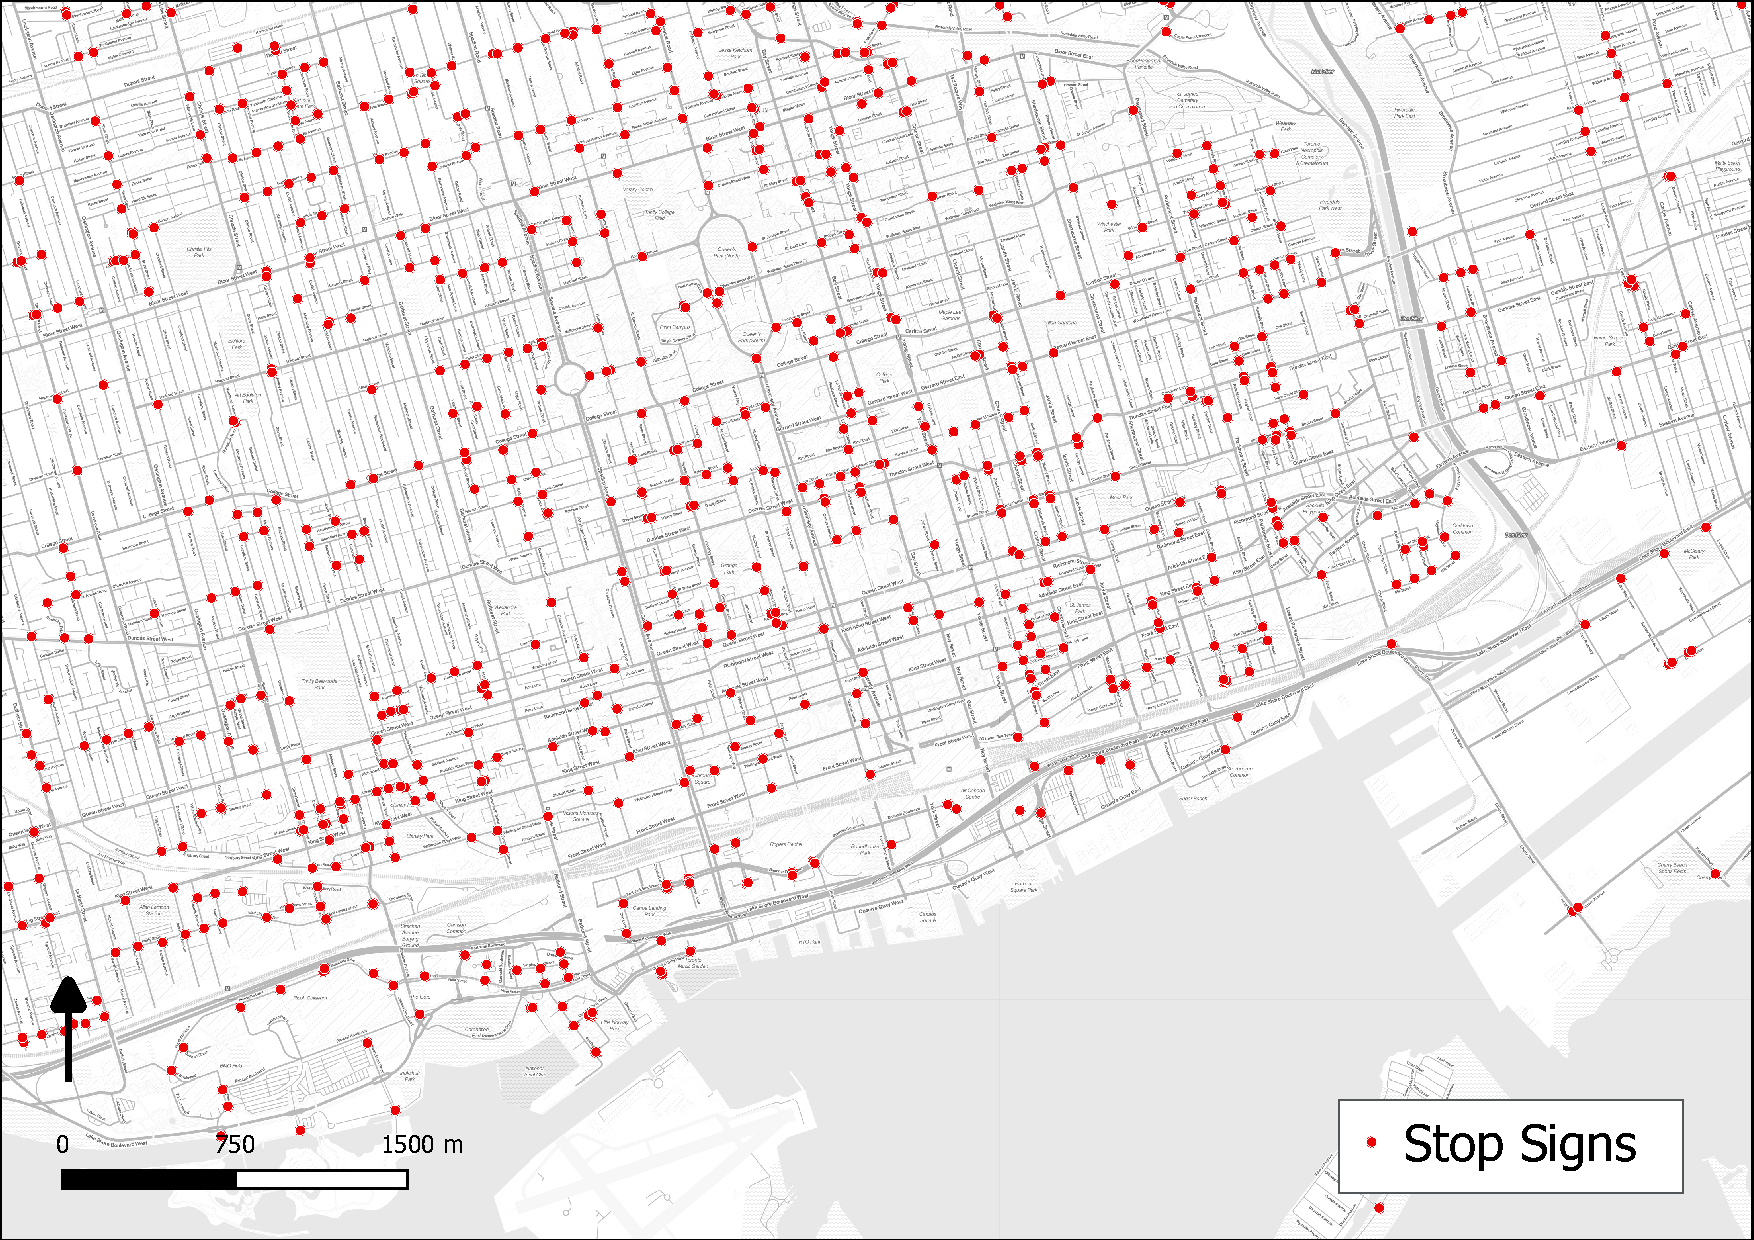
\includegraphics[width=4in, center]{coordinates_map}
  \caption{Map of stop sign locations in Toronto, Ontario, from OpenStreetMap}
  \label{fig:map-stop-signs}
\end{figure}

\begin{figure}[H]
  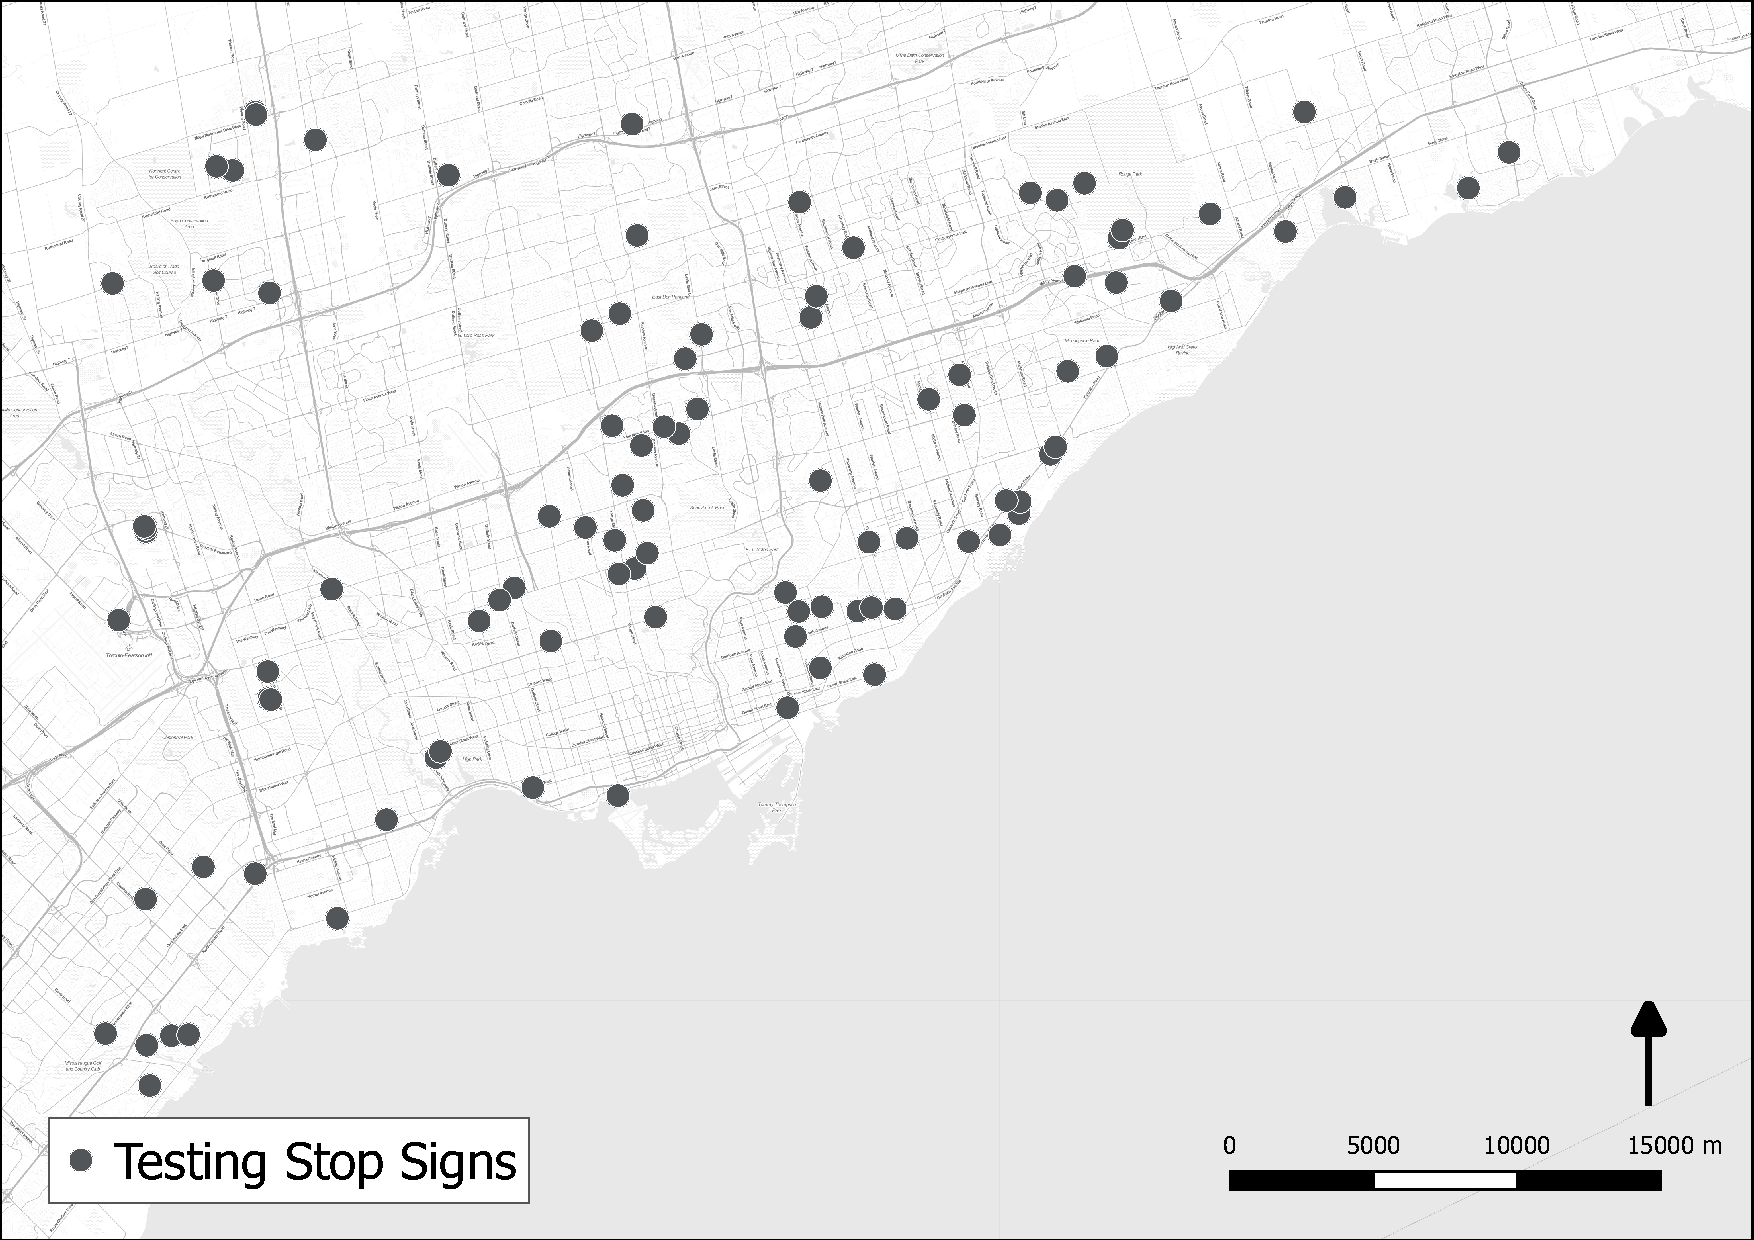
\includegraphics[width=4in, center]{coordinates_random_map}
  \caption{Map of randomly selected testing stop signs in Toronto, Ontario, from OpenStreetMap}
  \label{fig:map-random}
\end{figure}

A total of 10401 stop sign locations were extracted from OpenStreetMap using the Overpass API on June 26, 2017. These locations  are shown in Figure \ref{fig:map-stop-signs}. A total of 99 locations were randomly selected to be used for GSV image extraction and performance evaluation. These randomly selected locations are shown in Figure \ref{fig:map-random}. Using the randomly selected locations, 99 GSV images were extracted using the GSV API. Out of the 99 GSV images, 19 were labeled positive (having a stop sign), and 80 were labeled negative (not having a stop sign). Figure \ref{fig:example-gsv-positive} shows a few examples of the positive images, and Figure \ref{fig:example-gsv-negative} shows a few examples of the negative images.

\begin{figure}[H]
  \begin{subfigure}[t]{1.5in}
    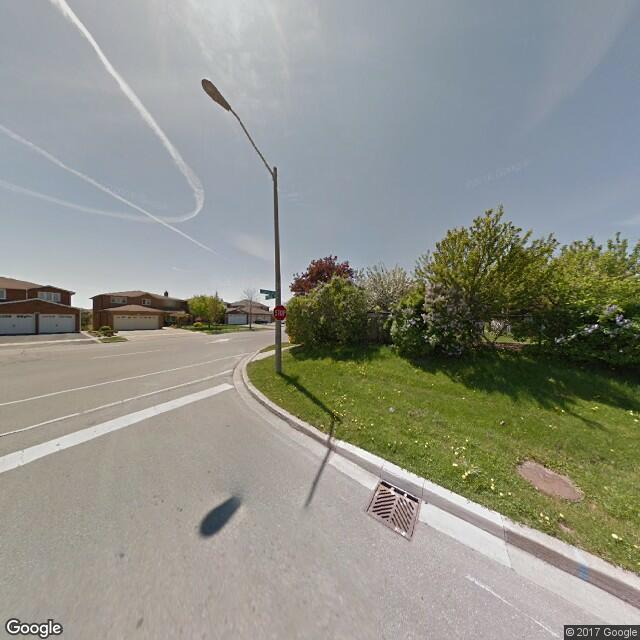
\includegraphics[height=1.5in]{gsv_1}
  \end{subfigure}
  \hfill
  \begin{subfigure}[t]{1.5in}
    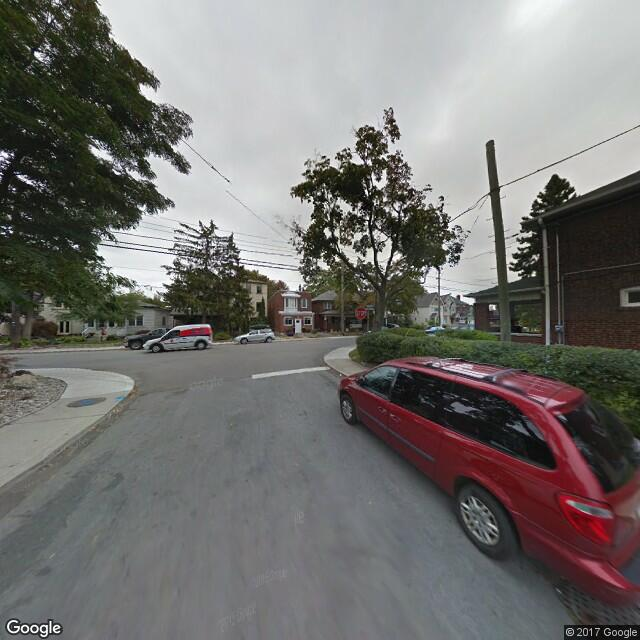
\includegraphics[height=1.5in]{gsv_14}
  \end{subfigure}
  \hfill
  \begin{subfigure}[t]{1.5in}
    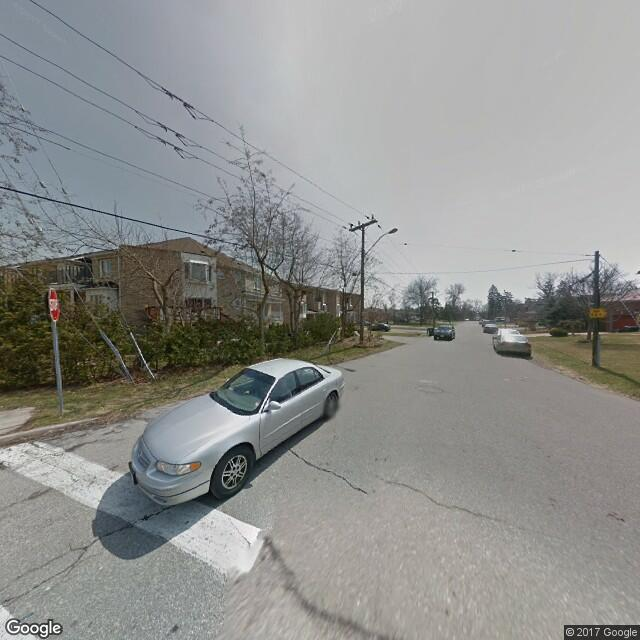
\includegraphics[height=1.5in]{gsv_18}
  \end{subfigure}
  \par\medskip
  \begin{subfigure}[t]{1.5in}
    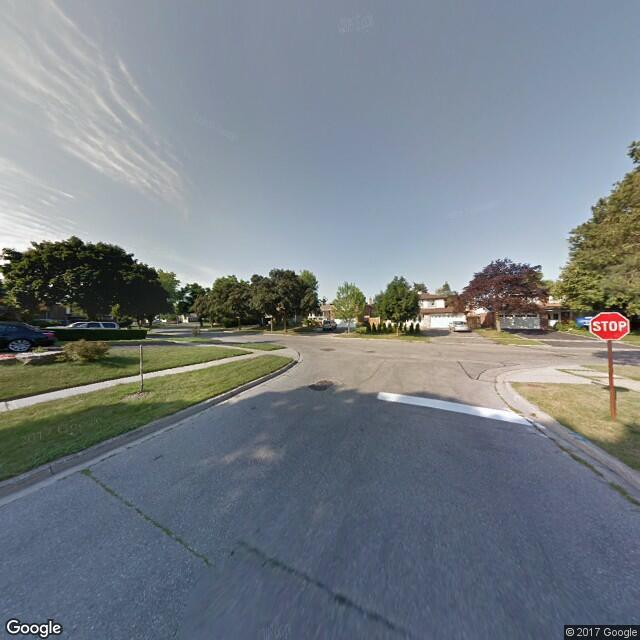
\includegraphics[height=1.5in]{gsv_38}
  \end{subfigure}
  \hfill
  \begin{subfigure}[t]{1.5in}
    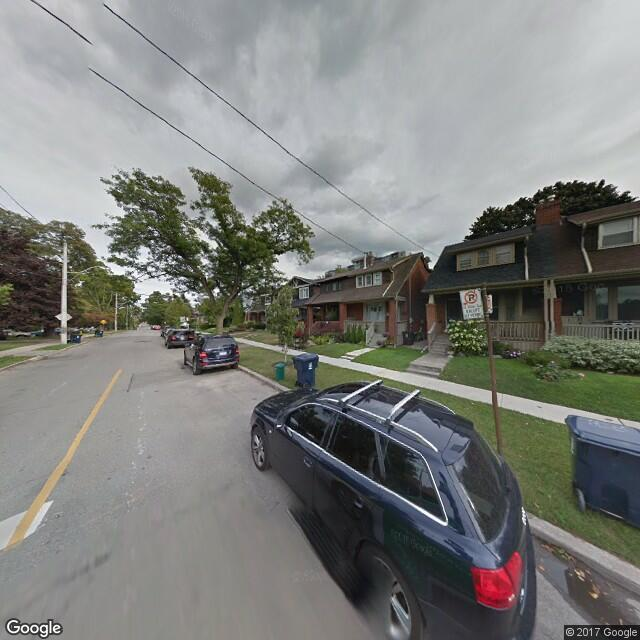
\includegraphics[height=1.5in]{gsv_85}
  \end{subfigure}
  \hfill
  \begin{subfigure}[t]{1.5in}
    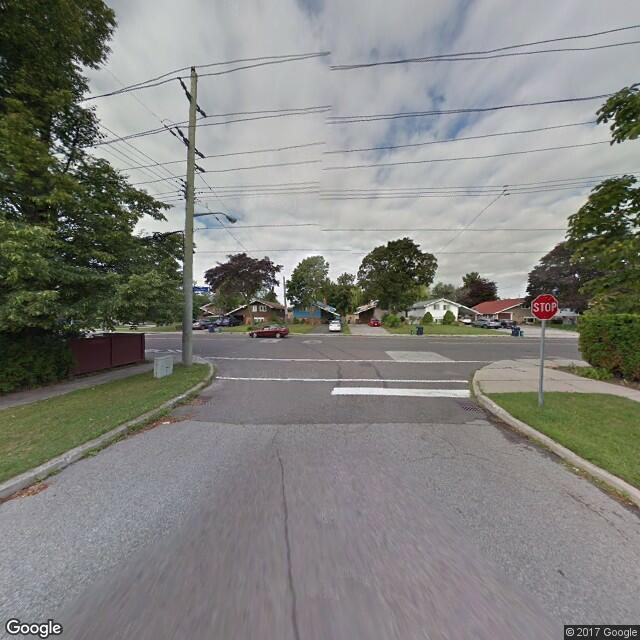
\includegraphics[height=1.5in]{gsv_87}
  \end{subfigure}
  \caption{Example of positive testing images}
  \label{fig:example-gsv-positive}
\end{figure}

\begin{figure}[H]
  \begin{subfigure}[t]{1.5in}
    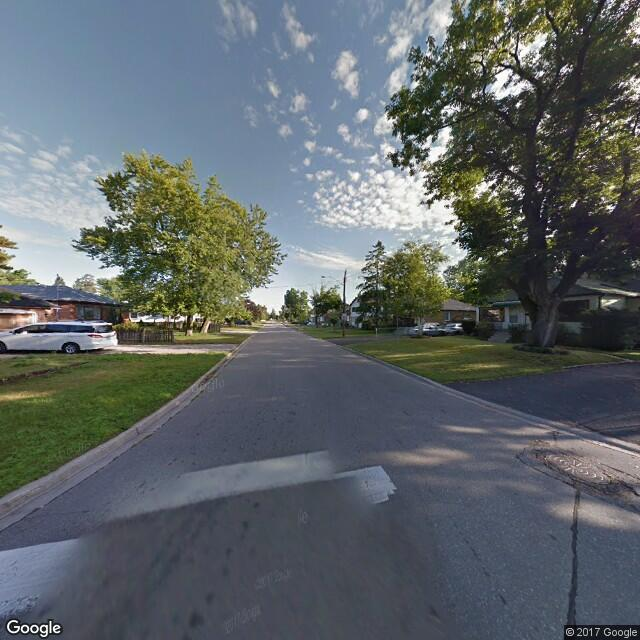
\includegraphics[height=1.5in]{gsv_0}
  \end{subfigure}
  \hfill
  \begin{subfigure}[t]{1.5in}
    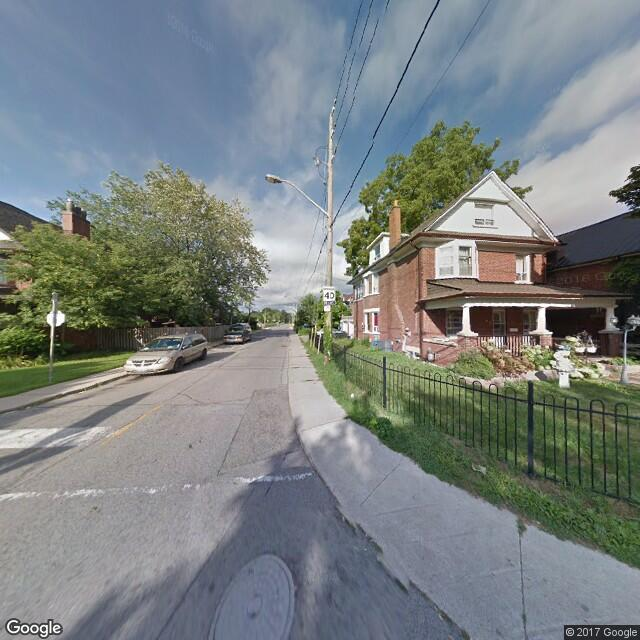
\includegraphics[height=1.5in]{gsv_13}
  \end{subfigure}
  \hfill
  \begin{subfigure}[t]{1.5in}
    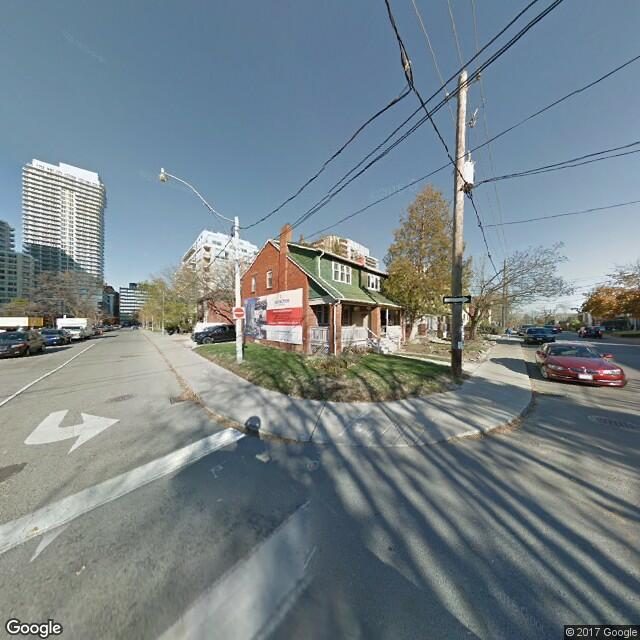
\includegraphics[height=1.5in]{gsv_2}
  \end{subfigure}
  \par\medskip
  \begin{subfigure}[t]{1.5in}
    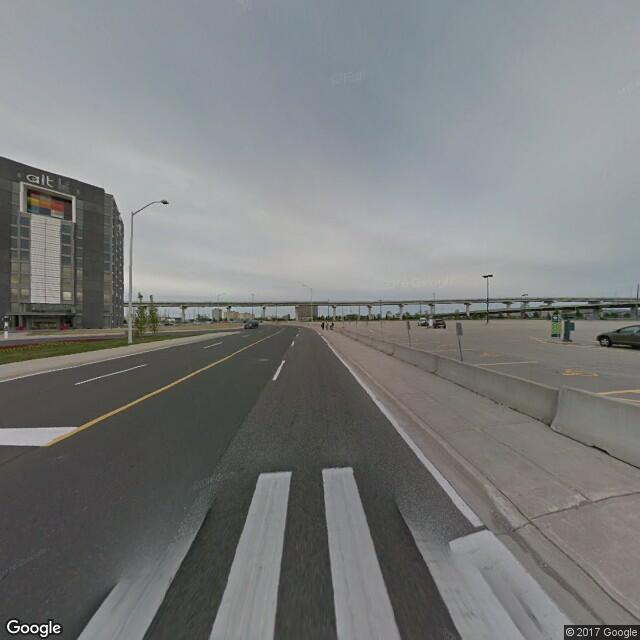
\includegraphics[height=1.5in]{gsv_29}
  \end{subfigure}
  \hfill
  \begin{subfigure}[t]{1.5in}
    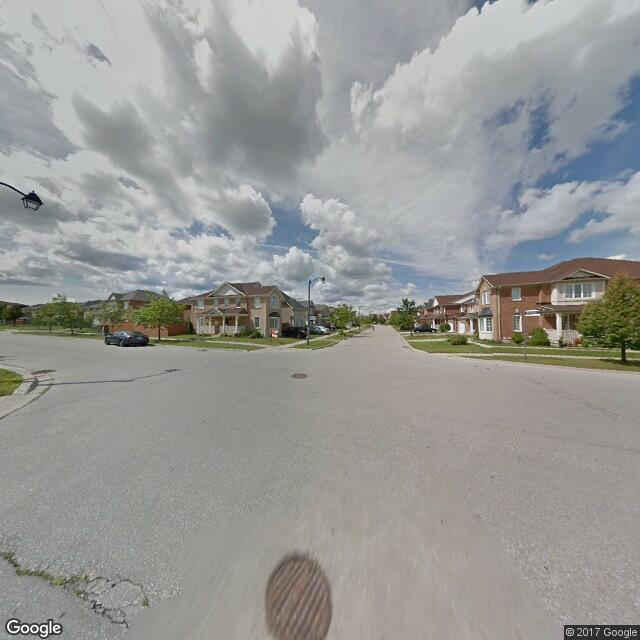
\includegraphics[height=1.5in]{gsv_47}
  \end{subfigure}
  \hfill
  \begin{subfigure}[t]{1.5in}
    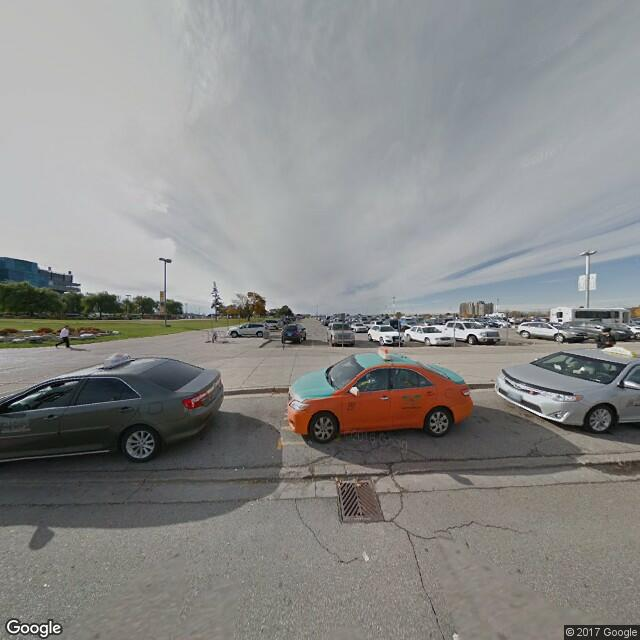
\includegraphics[height=1.5in]{gsv_51}
  \end{subfigure}
  \caption{Example of negative testing images}
  \label{fig:example-gsv-negative}
\end{figure}

The HCC stop sign model was able to only detect 6 of the positive images, and had a misclassification in 1 of the negative images. The detection ratio value was approximately 0.316, and the false positive ratio value was 0.0125. The detected stop signs are shown in Figure \ref{fig:detected} and the misclassified stop sign is shown in Figure \ref{fig:misclass}

\begin{figure}[H]
  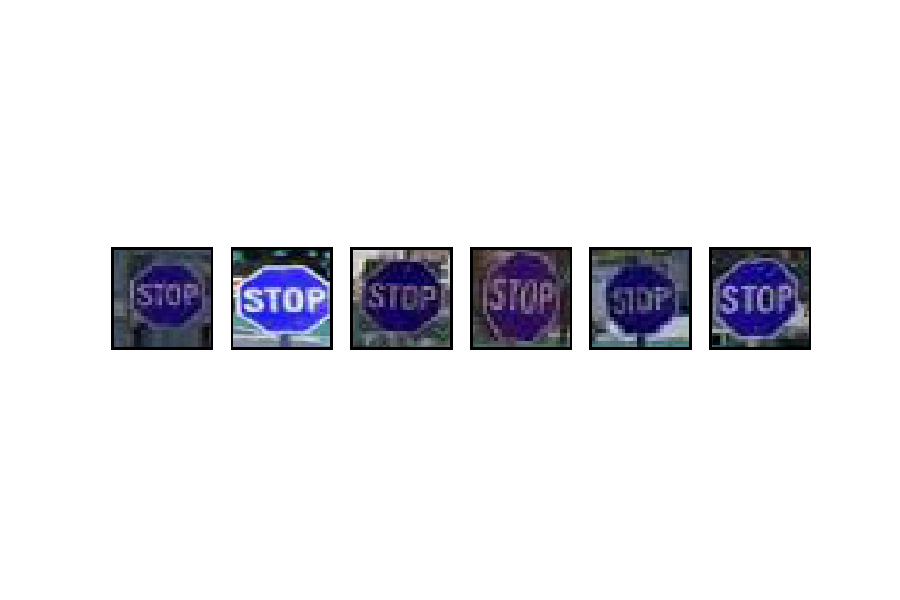
\includegraphics[width=4in, center]{positive_detections}
  \caption{Detected stop signs in the positive images}
  \label{fig:detected}
\end{figure}

\begin{figure}[H]
  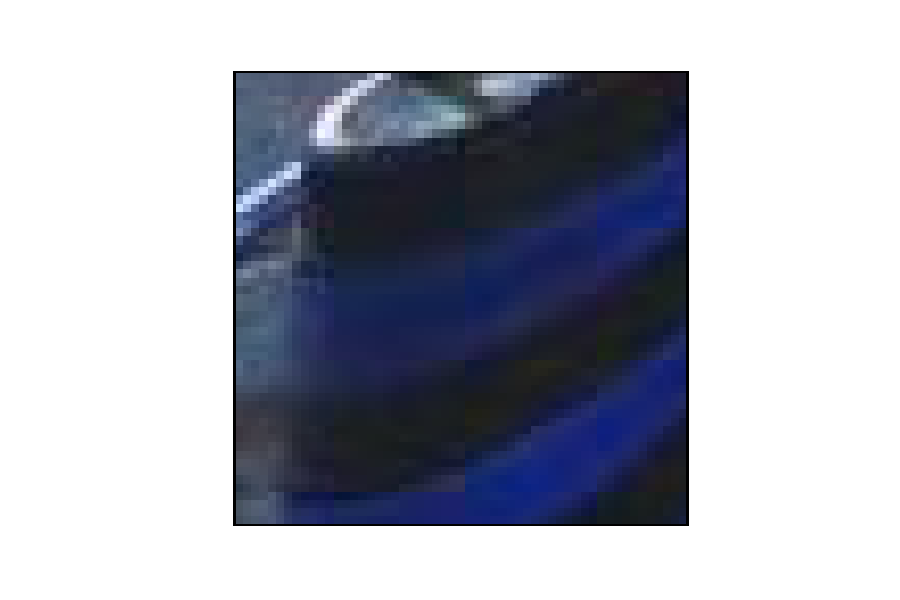
\includegraphics[width=2in, center]{negative_detections}
  \caption{Misclassified stop sign in the negative images}
  \label{fig:misclass}
\end{figure}

% ==========
% Discussion
% ==========
\section{Discussion} \label{discussion}

The HCC stop sign model performed well for negative images (false positive ratio value of 0.0125), but had difficulty detecting stop signs in positive images (detection ratio value of 0.316). The HCC algorithm did not account for color, and extreme distortions of the stop signs in the GSV images, as the Haar-like features were calculated on only grayscale images according to the Viola and Jones algorithm. Some stop signs in the positive images were also further away, and may cause reduce image quality and different feature values being calculated. However, the rapid classification times of the HCC stop sign model provides a potential for object detection in real-time and big data. The massive quantities of real-time and big data make it often impractical to train and classify highly accurate algorithms images on demand due to the long training times. The HCC algorithm can train a classifier that can be used to classify images in real-time, and is appropriate when there are massive quantities of data due to the optimized efficiencies of the integral images and cascaded classifiers. In general, the HCC algorithm relies on the patterns of the varying grayscale intensities of images, but if these images are do not have enough pattern variance, then the resulting classifier is expected to perform poorly. Thus, the grayscale intensities are affected by distortions, angle of view, and image quality of the object of interest. For example, when viewing the stop signs from behind, the grayscale intensities differ greatly from the front of the stop sign, and therefore is likely to not be detected. A simple solution for the issue of viewing angles is to train another classifier to detect particular angles in which the object differs greatly, and classify the detection as the same object. This may also be applied to different distortions, and image qualities, but may result in higher false positives. The following points were identified as important to using the HCC algorithm for stop sign detection:

\begin{enumerate}
  \item \textbf{Dynamic appearance}: the object's appearance changes greatly depending on distortions, viewing angles, and image quality, which may lead to the object being undetectable
  \item \textbf{Rapid detection}: the HCC can detect objects in real-time, which may be practical for filtering large datasets for objects of interest, before performing manual evaluation
  \item \textbf{Ensembling}: multiple HCCs can be combined together easily to provide more accurate object detection when dealing with dynamic object appearances due to the fast classification speed
\end{enumerate}

% ==========
% Conclusion
% ==========
\section{Conclusion} \label{conclusion}

This paper detailed a small experiment on stop detection in GSV images using the HCC algorithm. An extensive review of background literature and algorithm implementation was done to improve understanding of the HCC based on the Viola and Jones algorithm. The experiment began with the extraction of stop sign locations to further collect GSV images for testing the performance of a pre-trained HCC stop sign model. A random selection of the collected GSV images was done to reduce the problem set to a more managable size for manual labelling. The performance evaluation measured the HCC stop sign model based on its ability to detect stop signs in GSV images, and to reject GSV images when stop signs did not exist in the image. The results showed that the HCC stop sign model had good performance in rejecting GSV images without stop signs, but poor performance when stop signs existed in GSV images. Although the detection performance was poor for this particular experiment, the advantage of the HCC algorithm lies in its ability to rapidly classify large quantities of images easily. This speed enables it to potentially be able to improve its performance by ensembling multiple HCCs to account for dynamic object appearance issues such as distortions, viewing angles, and image quality. With higher detection rates, there is potential for object detection algorithms to extract valuable and unique geospatial data from images with location metadata such as street level features, civilians, and human activity.

% ================
% Acknowledgements
% ================

\section*{Acknowledgements}

I would like to thank Dr. Wai Yeung Yan for providing me the freedom to explore the experiment documented in this paper as an alternative to the term project for the course. I would also like to thank Github user \textit{markgaynor} for open sourcing the Haar Cascade Classifier model and training data used in this paper's experiment under the MIT license.

% ============
% Bibliography
% ============
\bibliographystyle{apa}
\bibliography{reference}

% ==========
% Appendices
% ==========
\appendix

\section{Integral Image Example} \label{integral-image-example}

\begin{figure}[H]
  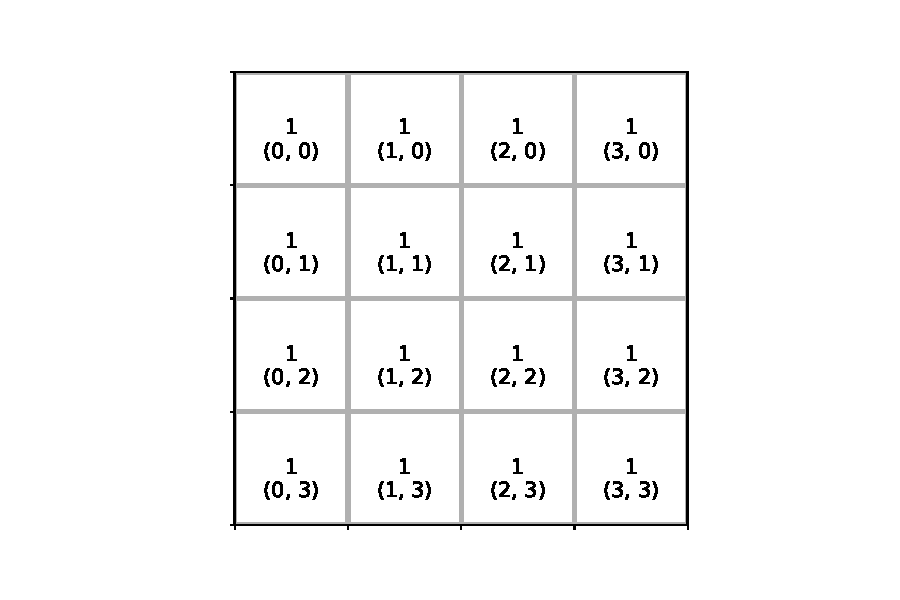
\includegraphics[center]{integral_i}
  \caption{Example of an image i}
  \label{fig:integral-i}
\end{figure}

Given an original image ii with 4 rows by 4 columns where each pixel has a value of 1 and coordinates are defined by $(x,y)(x,y)$ (Figure \ref{fig:integral-i}).

\begin{figure}[H]
  \centering
  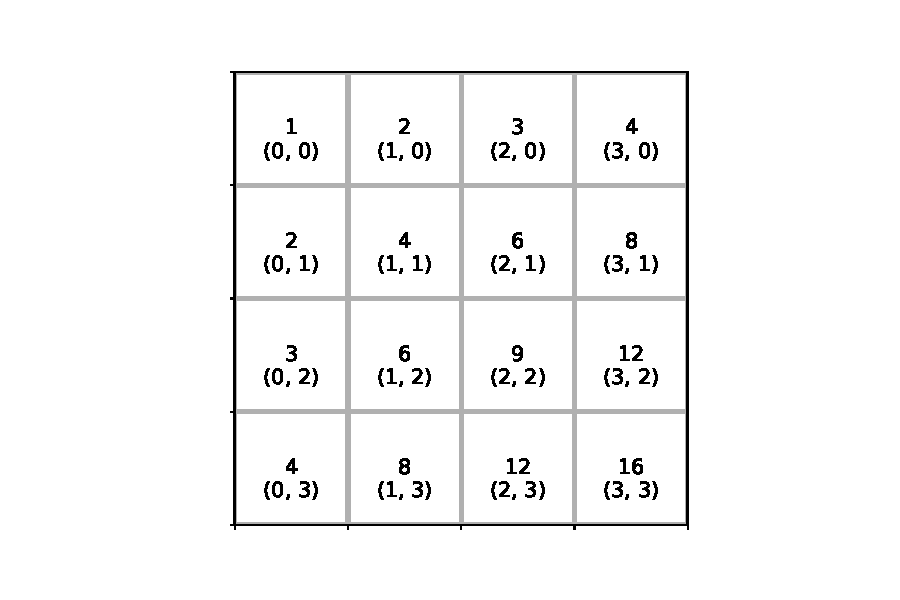
\includegraphics[center]{integral_ii}
  \caption{Example of an integral image ii}
  \label{fig:integral-ii}
\end{figure}

The integral image ii for the first two rows and columns can be computed as follows (Figure \ref{fig:integral-ii}):

\begin{itemize}
  \item Row 1, Column 1: $ii(1,1)=i(1,1)ii(1,1)=i(1,1)$
  \item Row 1, Column 2: $ii(1,2)=i(1,1)+i(1,2)=1+1=2$
  \item Row 2, Column 1: $ii(2,1)=i(1,1)+i(2,1)=1+1=2$
  \item Row 2, Column 2: $ii(2,2)=i(1,1)+i(1,2)+i(1,3)+i(1,4)=1+1+1+1=4$
\end{itemize}

\begin{figure}[H]
  \centering
  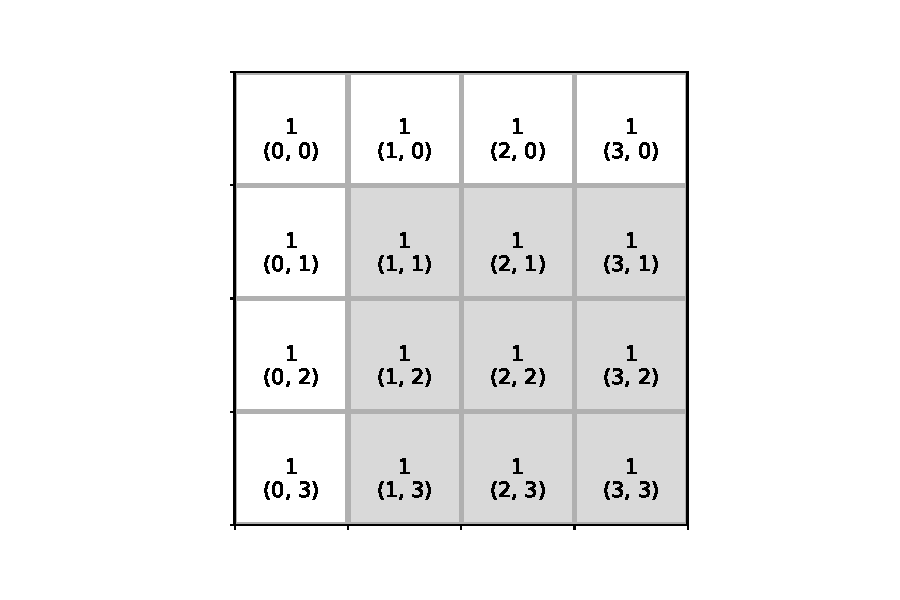
\includegraphics[center]{integral_i_rectangle}
  \caption{Example of a 3 by 3 rectangular region}
  \label{fig:integral-i-rectangle}
\end{figure}

A 3 by 3 rectangular region in gray for the original image, which requires 9 array accesses to calculate the sum of 9, is given (Figure \ref{fig:integral-i-rectangle}):

\begin{itemize}
  \item Bottom-left corner of region: $x_1,y_1=1,1$
  \item Top-left corner of region: $x_2,y_2=3,3$
\end{itemize}

\begin{figure}[H]
  \centering
  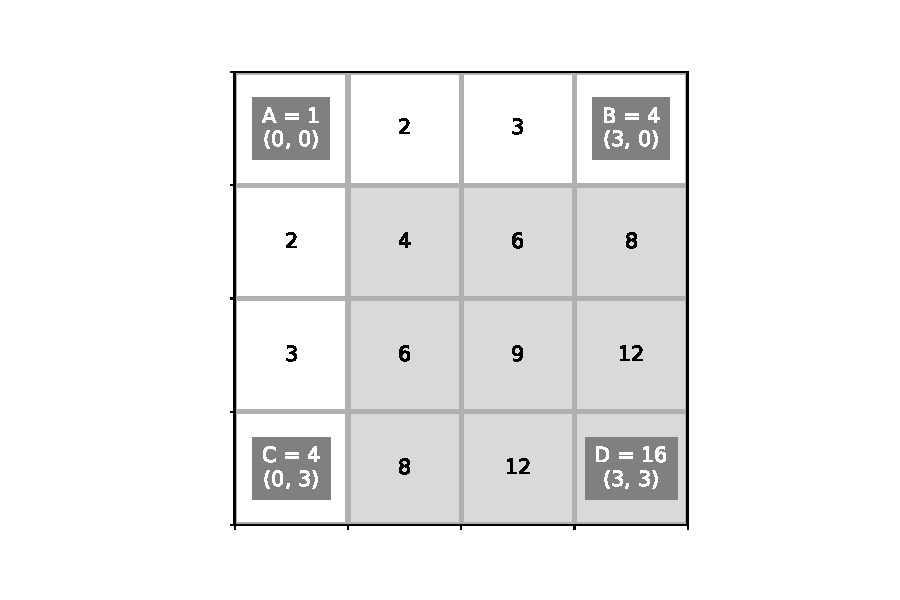
\includegraphics[center]{integral_ii_rectangle}
  \caption{Example of rectangular sum using an integral image}
  \label{fig:integral-ii-rectangle}
\end{figure}

The integral image can be used to calculate the sum of 9 with 4 array accesses instead (Figure \ref{fig:integral-ii-rectangle}):

\begin{itemize}
  \item Recall that $x_1, y_1 = 1,1$ and $x_2, y_2 = 3,3$
  \item $A = ii(x_1 - 1,y_1 - 1) = ii(1 - 1, 1 - 1) = ii(0, 0) = 1$
  \item $B = ii(x_2,y_1 - 1)=ii(3, 1 - 1) = ii(3, 0) = 4$
  \item $C = ii(x_1 - 1, y_2) = ii(1-1,3) = ii(0, 3) = 4$
  \item $D = ii(x_2,y_2)=ii(3,3)=16$
  \item $Si(1, 1, 3, 3) = D - B - C + A = 16 - 4 - 4 + 1 = 9$
\end{itemize}

\section{Overpass API URL Structure} \label{overpass-api-url-structure}

An Overpass API request consisted of a base URL: 

\begin{verbatim}
http://overpass-api.de/api/interpreter
\end{verbatim}

and a data query string \textit{ql} after this base URL:

\begin{verbatim}
http://overpass-api.de/api/interpreter?data=ql
\end{verbatim}

\section{Google Street View URL API Structure} \label{google-street-view-url-structure}

A GSV API request consisted of a base URL:

\begin{verbatim}
https://maps.googleapis.com/maps/api/streetview
\end{verbatim}

and a data query string \textit{params} after this base URL:

\begin{verbatim}
https://maps.googleapis.com/maps/api/streetview?params
\end{verbatim}

The GSV API metadata was checked to see if a requested image exists before downloading using a seperate base URL:

\begin{verbatim}
https://maps.googleapis.com/maps/api/streetview/metadata
\end{verbatim}